% !tex root=./main.tex

\section{Probabilistic Context-Free Grammars}
\label{app:pcfg}

We show the \emph{astronomers} \gls{PCFG} in \cref{fig:app/pcfg/astronomers}.
\Cref{fig:experiments/pcfg/vimco_q_samples} shows samples from an inference network trained with \gls{VIMCO} with $K = 20$, conditioned on the sentence $x = $ ``astronomers saw stars with telescopes''.
\Cref{fig:experiments/pcfg/production_probs} shows production probabilities of the non-terminal NP learned by \gls{VIMCO} and \gls{WS} with $K = 20$.
\begin{figure}[htb]
  \begin{align*}
    \text{S} \to&\,\, \text{NP}\,\text{VP}\,(1.0) \\
    \text{NP} \to&\,\, \text{NP}\,\text{PP}\,(0.4) | \text{astronomers}\,(0.1) | \text{ears}\,(0.18) | \\
    &\,\, \text{saw}\,(0.04) | \text{stars}\,(0.18) | \text{telescopes}\,(0.1) \\
    \text{VP} \to&\,\, \text{V}\,\text{NP}\,(0.7) | \text{VP}\,\text{PP}\,(0.3) \\
    \text{PP} \to&\,\, \text{P}\,\text{NP}\,(1.0) \\
    \text{P} \to&\,\, \text{with}\,(1.0) \\
    \text{V} \to&\,\, \text{saw}\,(1.0).
  \end{align*}
  \caption{\emph{The astronomers \acrshort{PCFG}} from \citet[Table 11.2]{manning1999foundations}. The terminals are $\{\text{astronomers}, \text{ears}, \text{saw}, \text{stars}, \text{telescopes}, \text{with}\}$, the non-terminals are $\{\text{S}, \text{NP}, \text{VP}, \text{PP}, \text{P}, \text{V}\}$ and the start symbol is S.
  Each row above lists production rules $\{n_i \to \zeta_j\}$ with the corresponding probabilities $p_{ij}$ in the format $n_i \to \zeta_1\,(p_{i1}) | \zeta_2\,(p_{i2}) | \cdots | \zeta_J\,(p_{iJ})$.}
  \label{fig:app/pcfg/astronomers}
\end{figure}
\begin{figure}[htb]
  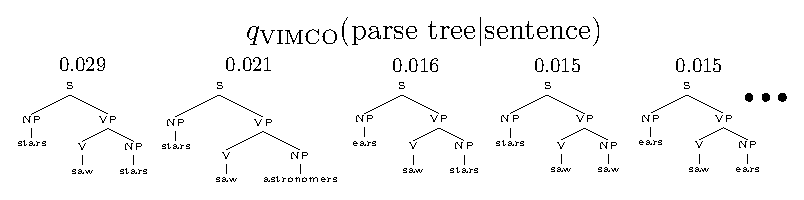
\includegraphics[scale=0.6]{figures/RRWS/pcfg/vimco_q_samples.eps}
  \caption{Samples from the inference network which was trained with \gls{VIMCO} with $K = 20$.}
  \label{fig:experiments/pcfg/vimco_q_samples}
  \vspace*{-2ex}
\end{figure}
\begin{figure}[htb]
  \centering
  \includegraphics[width=0.7\linewidth]{figures/RRWS/pcfg/np_probs.pdf}
  \caption{Production probabilities for the non-terminal NP learned via \gls{WS} and \gls{VIMCO} with $K = 20$.}
  \label{fig:experiments/pcfg/production_probs}
  \vspace*{-2ex}
\end{figure}


\section{Attend, Infer, Repeat}
\label{app:air}

\Gls{AIR} is a model with many components and might be difficult to understand if not described explicitly.
Here, we outline details of our implementation and provide pseudo-code for the inference (\cref{algo:air_inference}) and generative models (\cref{algo:air_generation}) in the case of continuous data and Gaussian data likelihood.

\begin{algorithm}[!h]
    \caption{Inference in \gls{AIR}}
    \label{algo:air_inference}
    \DontPrintSemicolon
    % \SetAlgoLined
    \SetKwInOut{Input}{Input}
    \SetKwInOut{Output}{Output}
    \SetSideCommentLeft
    \Input{Image $\bm{x}$,\\ maximum number of inference steps $N$}
    $\bm{h}_0, \bm{z}^\text{what}_0, \bm{z}^\text{where}_0$ = initialize()\\
    \For{$n \in [1, \dots, N]$}{
        $\bm{w}_n, \bm{h}_n = R_\phi \left( \bm{x}, \bm{z}^\text{what}_{n-1}, \bm{z}^\text{where}_{n-1}, \bm{h}_{n-1} \right)$\\
        $p_n \sim \mathrm{Bernoulli} (p \mid \bm{w}_n)$\\
        \If{$p_n = 0$}{
            break
        }
        $\bm{z}^\text{where}_n \sim q_\phi^\text{where} \left( \bm{z}^\text{where} \mid \bm{w}_n \right)$\\
        $\bm{g}_n = \text{STN} \left( \bm{x}, \bm{z}^\text{where}_n \right)$\\
        $\bm{z}^\text{what}_n \sim q_\phi^\text{what} \left( \bm{z}^\text{what} \mid \bm{g}_n \right)$\\
    }
\Output{$\bm{z}^\text{what}_{1:n}$, $\bm{z}^\text{where}_{1:n}$, $n$}
\end{algorithm}
\begin{algorithm}[!h]
    \caption{Generation in \gls{AIR}}
    \label{algo:air_generation}
    \DontPrintSemicolon
    \SetKwInOut{Input}{Input}
    \SetKwInOut{Output}{Output}
    \SetSideCommentLeft
    \Input{$\bm{z}^\text{what}_{1:n}$, $\bm{z}^\text{where}_{1:n}$, $n$}
    $\bm{y}_0 = \bm{0}$\\
    \For{$t \in [1, \dots, n]$}{
        $\hat{\bm{g}}_t = h_\theta^\text{dec} \left( \bm{z}^\text{what}_t \right)$\\
        $\bm{y}_t = \bm{y}_{t-1} + \text{STN}^{-1} \left( \hat{\bm{g}}_t, \bm{z}^\text{where}_t \right)$\\
    }
    $\hat{\bm{x}} \sim \mathrm{Normal} \left(\bm{x} \mid \bm{y}_n, \sigma^2_x \bm{I} \right)$\\
    \Output{$\hat{\bm{x}}$}
\end{algorithm}
\vspace*{-2ex}

\section{Gaussian Mixture Model}
\label{app:gmm}

\subsection{Control Variates}
Here, we present the architectures for the \acrshort{REBAR}/\acrshort{RELAX} control variate used in the \gls{GMM} experiment.

The reparameterized sampling of Gumbels and conditional Gumbels is described by \citet[Appendix C]{tucker2017rebar} and \citet[Appendix B]{grathwohl2018backpropagation}.
In the following, we describe architectures used for the \gls{GMM} experiment (\cref{sec:experiments/gmm}).

\Acrshort{REBAR} proposes the following architecture for the control variate $c_\rho(g_{1:K})$:
\begin{align}
    c_\rho^{\acrshort{REBAR}}(g_{1:K}) = \rho_1 \log\left(\frac{1}{K} \sum_{k = 1}^K \frac{p_\theta(\mathrm{sm}(g_k / e^{\rho_2}), x)}{q_\phi(\mathrm{sm}(g_k / e^{\rho_2}) \given x)}\right), \label{eq:rebar-c}
\end{align}
where $\rho = (\rho_1, \rho_2)$, and $\mathrm{sm}$ refers to the softmax function.
While the functional form of \cref{eq:rebar-c} suggests that it will be highly correlated with $\log(\frac{1}{K} \sum_{k = 1}^K w_k)$, the terms \glspl{PMF} in the fraction are undefined due to the softmax.
A straightforward fix is to evaluate ``a soft \gls{PMF}'' instead:
\begin{align*}
    &p_\theta(\mathrm{sm}(g_k / e^{\rho_2}), x) \\
    &= p_\theta(\mathrm{sm}(g_k / e^{\rho_2})) p(x \given \mathrm{sm}(g_k / e^{\rho_2})) \\
    &= \mathrm{Categorical}(\mathrm{sm}(g_k / e^{\rho_2}) \given \mathrm{sm}(\theta)) \cdot \\
    & \qquad\mathrm{Normal}(x \given \mu_{\mathrm{sm}(g_k / e^{\rho_2})}, \sigma_{\mathrm{sm}(g_k / e^{\rho_2})}^2) \\
    &\approx  \mathrm{sm}(g_k / e^{\rho_2})^\intercal \mathrm{sm}(\theta) \cdot \\
    & \qquad \mathrm{Normal}(x \given \mu^\intercal \mathrm{sm}(g_k / e^{\rho_2}), (\sigma^2)^\intercal \mathrm{sm}(g_k / e^{\rho_2})), \\
    &q_\phi(\mathrm{sm}(g_k / e^{\rho_2}) \given x) \\
    &= \mathrm{Categorical}(\mathrm{sm}(g_k / e^{\rho_2}) \given \mathrm{sm}(\eta_\phi(x))) \\
    &\approx \mathrm{sm}(g_k / e^{\rho_2})^\intercal \mathrm{sm}(\eta_\phi(x)).
\end{align*}
Optimization of the log-temperature $\rho_2$ is highly sensitive as low values can make the training unstable.

\Acrshort{RELAX} proposes using an arbitrary neural network for $c_\rho(g_{1:K})$.
Due to the symmetry in the arguments, we pick the following for the \gls{GMM} experiment:
\begin{align}
    c_\rho^{\acrshort{RELAX}}(g_{1:K}) = \frac{1}{K} \sum_{k = 1}^K \acrshort{MLP}_\rho([x, g_k]), \label{eq:relax-c}
\end{align}
where the architecture of the \gls{MLP} is $(1 + C)$-$16$-$16$-$1$ (with the $\tanh$ nonlinearity between layers) and $\rho$ are the weights are its weights.
This architecture is---unlike the one in \cref{eq:rebar-c}---well-defined for all inputs.
A drawback of using such control variate is that it can start out not being very correlated with $\log(\frac{1}{K} \sum_{k = 1}^K w_k)$.

\Acrshort{RELAX} also proposes using a summation of the free-form control variate like the one in \cref{eq:relax-c} and a more correlated control variate in \cref{eq:rebar-c}.

We have tried all architectures and found that \cref{eq:relax-c} leads to the most stable and best training.

Using \acrshort{REBAR}/\acrshort{RELAX} for more complicated models is possible, however designing an architecture that is highly correlated with the high-variance term and stable to train still remains a challenge.

\begin{figure*}[!htb]
  \centering
  \includegraphics[width=\textwidth]{figures/RRWS/gmm/errors_just_std.pdf}
  \caption{
    Standard deviation of gradient estimator of $\phi$ for \gls{GMM}.
    Median and interquartile ranges from $10$ repeats shown.
    \Gls{WW} and \gls{WS} have lower-variance gradient estimators of $\phi$ than \gls{IWAE} except \gls{VIMCO}, as they avoid the high-variance term \circled{1} in \eqref{eq:iwae-reinforce}.
    This is a necessary, but not sufficient, condition for efficient learning, with other factors being gradient direction and the ability to escape local optima.
    The standard deviation of $\phi$'s gradient estimator is given by $\frac{1}{D_\phi} \sum_{d = 1}^{D_\phi} \std(g_d)$ where $g_d$ is the $d$th (out of $D_\phi$) element of one of $\phi$'s gradient estimators (e.g. \cref{eq:iwae-reinforce} for \acrshort{REINFORCE}) and $\std(\cdot)$ is estimated using $10$ samples.
  }
  \label{fig:gmm_just_std}
\end{figure*}

\subsection{Additional Results}
\label{app:gmm/additional}

Here, we include additional \gls{GMM} experiments:
one for studying $\phi$'s gradient variance (\cref{fig:gmm_just_std}),
the other for comparing performances of the generative model and inference networks when $\theta$ is initialized closer to $\theta^*$ than in the main paper (\cref{fig:gmm_init_near}).

\Gls{WW} and \gls{WS} have lower variance gradient estimators than \gls{IWAE}, except \gls{VIMCO}.
%
This is because $\phi$'s gradient estimators for \gls{WW} and \gls{WS} do not include the high-variance term \circled{1} in \cref{eq:iwae-reinforce}.
%
This is a necessary but not sufficient condition for efficient learning with other important factors being gradient direction and the ability to escape local optima.
%
Employing the Concrete distribution gives low-variance gradients for $\phi$ to begin with, but the model learns poorly due to the high gradients bias (due to high temperature hyperparameter).

In \cref{fig:gmm_init_near}, we initialize $\theta$ so that the mixture probabilities are constant.
This means that the data bias is smaller than in the main paper's setting.
With smaller data bias, we expect \gls{WS} to perform better.
This is empirically verified since \gls{WS} outperforms other methods, including \gls{WW}.


\begin{figure*}[!ht]
  \centering
  \includegraphics[width=\textwidth]{figures/RRWS/gmm/errors_near.pdf}
  \vspace*{-4ex}
  \caption{
    \Gls{GMM} training when $p_\theta(x)$ is close to $p_{\theta^*}(x)$.
    \Gls{WS} outperforms other methods including \gls{WW} in generative model (top) and inference network (middle) learning.
    \Gls{VIMCO} has the lowest gradient variance (bottom) but still performs worse than \gls{WS} and results in worsening of the inference network as number of particles is increased.
  }
  \label{fig:gmm_init_near}
  \vspace*{-2ex}
\end{figure*}

\section{Sigmoid Belief Networks}
\label{app:sigmoid_belief_nets}

In \cref{fig:sbn}, we show training of sigmoid belief networks with three stochastic layers with the same architecture as in \citet{Mnih2016variational}.
We additionally drive number of particles up to $K = 5000$ and include \gls{KL} plots.
We find that in high particle regimes, model learning is virtually the same for \gls{WW} and \gls{VIMCO}.
However, \gls{WW} outperforms \gls{VIMCO} in terms of inference network learning.

\begin{figure*}[!ht]
  \includegraphics[width=\textwidth]{figures/RRWS/discrete_vae/rws_baselines.pdf}
  \vspace*{-4ex}
  \caption{
    Training of sigmoid belief nets.
    \emph{(Left)}
    Training curves:
    \gls{WW} learns faster than \gls{VIMCO} but results in equal or slightly worse end test log likelihood.
    \emph{(Middle)}
    Log evidence values at the end of training:
    \gls{VIMCO} is slightly better than \gls{WW} in low-particle regimes but virtually the same in high-particle regimes.
    \emph{(Right)}
    \gls{KL} divergence at the end of training:
    \gls{WW} results in much lower \gls{KL} divergence than \gls{VIMCO}.
  }
  \label{fig:sbn}
  \vspace*{-2ex}
\end{figure*}

\section{Discrete VAEs}
\label{app:dvae}

Rolfe 2016 \citep{Rolfe2016dvae} introduces discrete \textsc{vae} (\textsc{dvae}).
It combines a prior over binary latent variables with an element-wise spike-and-X smoothing transformation, allowing approximate marginalization of the discrete variables.
This results in a continuous relaxation of discrete variables and a low-variance gradient estimator.
\citet{Vahdat2018dvaepp} replaced the original transformation with an overlapping exponential transformation, leading to a yet lower-variance gradient estimator.
While both approaches produce relaxed binary variables, the relaxation is  significantly less tight (\cite{Vahdat2018dvaepp}, Appendix C, Figure 5.) then the \textsc{concrete} of \cite{Jang2017categorical,Maddison2017concrete}
Both approaches require analytical inverse \textsc{cdf}s of the smoothing transformations, a shortcoming addressed by \citet{Vahdat2018dvaehash} --- it also leads to a tighter relaxation than its predecessors, however no comparison to \textsc{concrete} is available.

\textsc{Dvae} was designed for undirected binary priors, \textit{e.g.}\ restricted Boltzmann machines (\textsc{rbm}), and it does not account for the case of categorical latent variables.
It is possible to construct a $d$-dimensional categorical variable from  $d-1$ binary variables via stick-breaking construction.
This process is slow, however, as it requires $\operatorname{\mathcal{O}}(d)$ sequential operations and cannot be parallelized.
Moreover, in the case of relaxed variables, the tightness of the derived relaxed categorical variable decreases exponentially with the number of dimensions.
This is a major issue in control flows: not only we have to evaluate all branches of the control flow, but the indicator variables that we multiply with outcomes of different branches become exponentially loose with the depth of the flow.


% \section{List of acronyms}
% \renewcommand{\glossarysection}[2][]{}
% \printglossary[type=\acronymtype]
